\section{Frameworks}

Al comienzo de la aparición de las aplicaciones web, los desarrolladores disponían únicamente de \gls{HTML}, \gls{JS} y \gls{CSS} para su implementación, sin ningún tipo de librería ni framework que les facilitará esta tarea. Se conoce como \emph{Vanilla JavaScript} al uso de JavaScript sin ningún tipo de librería ni framework. Con el aumento tanto en número como en complejidad de estas aplicaciones, se hizo necesario disponer de herramientas que facilitarán el desarrollo de estas.

Así comenzaron a surgir diferentes herramientas y frameworks que facilitaban las tareas de programación tanto en el lado de la lógica de negocio como en el apartado visual.

\subsection{jQuery}

jQuery\footnote{\url{https://jquery.com/}} fue y sigue siendo una de las librerías más usada en el mundo del desarrollo web. Esta librería tiene como objetivo facilitar algunas de las deficiencias que nos encontramos a la de programar con JavaScript.

Con jQuery conseguimos simplificar el acceso a los nodos del árbol \emph{DOM} que el navegador crea a partir de nuestro \gls{HTML}, consiguiendo una sintaxis mas clara, fácil de recordar y además compatible con todos los navegadores. Por ejemplo:

\begin{lstlisting}[style=htmlcssjs,frame=tlrb,xleftmargin={0.2cm}]
  // Vanilla JavaScript
  var elem = document.getElementById("miElemento");

  //jQuery
  var elem = \$("#miElemento");
\end{lstlisting}

También proporciona herramientas útiles como métodos específicos para realizar llamadas \emph{AJAX}, es decir, llamadas desde la aplicación web que se ejecuta en el navegador al servidor de manera asíncrona utilizando el protocolo \gls{HTTP}.

jQuery ha supuesto el punto de partida de muchos otros frameworks y complementos, lo que hace que tenga aún más valor. Ya que hablamos de la importancia de jQuery como base para otros proyectos, sería injusto no mencionar a \emph{underscoreJS}\footnote{\url{http://underscorejs.org/}}, otra librería que ha venido a suplir algunas cadencias de JavaScript.

Mas tarde, se lanzo jQuery UI\footnote{\url{http://jqueryui.com/}}, que consistía en un conjunto de herramientas y facilidades tanto CSS como JavaScript para la creación de interfaces de usuario. A su vez, de jQuery UI\footnote{\url{http://jquerymobile.com/}} surgió jQuery Mobile, una versión adaptada a dispositivos móviles que por aquella época empezaban cobrar mayor importancia.

\subsection{Framework CSS}

\cite{BootstrapFoundation,BestFramCSS} Con el paso de los años, el diseño de las páginas a ido haciéndose cada más y más complejo. Las diferentes versiones de \gls{HTML} y de \gls{CSS} han ido introduciendo nuevas opciones en este sentido, lo que aún siendo necesarias, a veces resultan insuficientes en el desarrollo de la página. Además de esto, la variedad de terminales desde los que se puede visualizar una página es también cada vez mayor, teniendo que pensar en el diseño según sea vista en un dispositivo móvil, una tablet, un PC, el navegador que se utiliza (ya que todos no reconocen los mismos parámetros), \ldots y no solo eso, también el tamaño de pantalla, la resolución, la orientación, \ldots. Si conseguimos que nuestro diseño se adapte a todos estos casos, podremos decir que el nuestro se trata de un diseño \emph{responsive}. Como nos podemos imaginar, el realizar un diseño \emph{responsive} requiere una cantidad de tiempo y recursos importante, ya que no solo debemos de implementar el estilo para diferentes usos, también es necesario probarlo.

Esta tarea de diseño ha sido facilitada con la aparición de lo que se conocen como \emph{frameworks \gls{CSS}}. Estos frameworks utilizan hojas de estilos creadas y testadas por equipos de desarrolladores y diseñadores con gran experiencias, listas para ser usadas como base en una maquetación web y no tener que partir desde cero. Una de la funcionalidades principales que suelen ofrecer, y que siempre a sido un dolor de cabeza para los diseñadores, razón por la que la destaco, son los \emph{grid}. Gracias ellos podemos dividir nuestra página en una especie de cuadrícula y sobre la que poder distribuir los elementos de nuestra página.

Aunque las ventajas de usar uno de estos frameworks son evidentes, también tienen ciertos inconvenientes a tener en cuenta antes de decidirnos a usarlos. En primer lugar es la limitación a la hora de personalizar el diseño, ya que partimos de uno ya creado y pensado para dar soporte a una gran cantidad de dispositivos, por lo que su implementación es compleja y modificarlo suele ser complicado. Otro inconveniente es el código del mismo framework. Lo más normal es que no se utilice todo lo que te ofrece el framework, pero aun así, será descargado por completo por el cliente. Según el tamaño y la conexión del cliente, esto puede ser un problema el cual, con la mejora de las conexiones, cada vez es menos importante.

\tipbox{
  Este tipo de frameworks suelen ofrecer un único núcleo y módulos separados los cuales implementan diferentes características. Así, podemos importar solo aquellos módulos que nos interesan, por ejemplo, el widget para el calendario o el módulo que maneja las tablas. También cuentan con versiones reducidas en los que el código esta ofuscado, consiguiendo reducir aún más el tamaño del código.
}

También tenemos que tener en cuenta la dificultad de aprendizaje de estos frameworks, lo que puede hacerlos poco atractivos para pequeños proyectos si no tenemos conocimientos y experiencia previa con ellos.

El anteriormente mencionado jQuery UI se considera un framework \gls{CSS}, pero han surgido durante los últimos años otros más potentes y más interesantes. Actualmente los dos más importantes se podría decir que son:

\begin{enumerate}
  \item Bootstrap\footnote{\url{getbootstrap.com}}: Desarrollado por Twitter, quien lo liberó como código abierto más tarde, se trata del framework \gls{CSS} más conocido y utilizado, siendo uno de los proyectos con más apoyo en Github\footnote{\url{https://github.com/}}. Se puede observar en la gráfica de debajo de estas líneas la diferencia de interés que despierta en comparación con Foundation, el otro gran framerwork \gls{CSS}, si tenemos en cuenta las búsquedas realizadas en Google. Sus puntos fuertes son su preocupación por la compatibilidad y la estabilidad (realizan test automáticos antes de publicar cualquier cambio en la rama principal del repositorio\footnote{\url{https://github.com/twbs/bootstrap}}), su sistema de \emph{Grid} y la gran comunidad que hay detrás. En su última versión utiliza tecnologías recientes como \gls{Sass}, implementan \emph{Flexbox} de \gls{CSS}, usan \glspl{mixin}\footnote{\url{http://getbootstrap.com/css/#mixins}} y hojas de estilos separadas para mejorar la escalabilidad \ldots.

  \begin{figure}[H]
\centering
    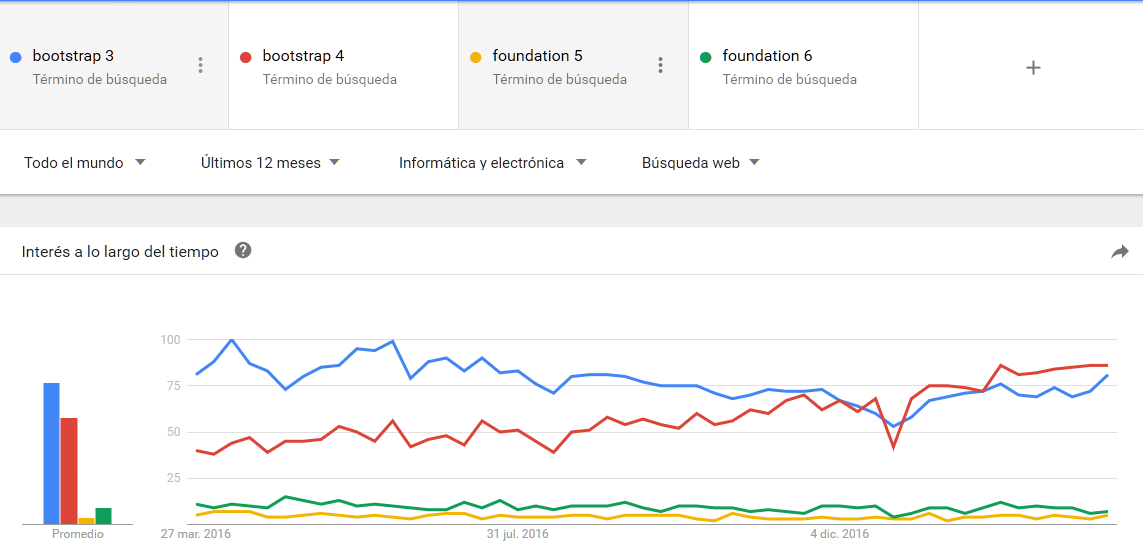
\includegraphics[width=0.8\textwidth]{Figures/ch1/frameworks/graph_frameworks_css}
    \caption{Busquedas mundiales de los dos frameworks CSS más importantes.}
  \end{figure}

  \item Foundation\footnote{\url{http://foundation.zurb.com/}}: Nos encontramos ante un framework que, aunque menos usado y apoyado, cuenta con una potencia similar a lo visto en Bootstrap. Al igual que este, hace uso de \gls{Sass}, \emph{Flexbox}, \glspl{mixin}, \ldots además de un sistema de \emph{Grid} considerado mejor que el de Bootstrap. Palidece, eso sí, si hablamos de compatibilidad y de estabilidad. Cuenta con una integración especial para \textbf{emails}, por lo que lo hace muy recomendable en caso de que nuestro diseño se tenga que adaptar al envío de correos. Todo esto hace que sea una alternativa igual de valida que Bootstrap.
\end{enumerate}

Aunque estos son los más importantes, existen otros muchos framework los cuales merece la pena mencionar como es Pure.CSS\footnote{\url{https://purecss.io/}}, cuya fuerza radica en su ligereza y sencillez, o Materialize\footnote{\url{http://materializecss.com/}}, enfocado en el estilo \emph{material design}.

\subsection{Framework Javascript}\label{subsec:frameworkJS}

 \cite{FramJSComp} Al igual que ha ocurrido con el diseño de las páginas, la lógica de negocio que se implementa en estas también a aumentado en complejidad. Se ha producido además un incremento de popularidad de las aplicaciones \gls{SPA}. En el desarrollo de este tipo de aplicaciones, trabajar solo con JavaScript se hace sumamente complicado, y  jQuery por si mismo no llega a cubrir todas las necesidades que iban surgiendo. Se hacia patente por tanto la necesidad de disponer de herramientas que facilitaran el desarrollo de estas páginas.

Estos framework proporcionan multitud de facilidades, pero hay que ser cauto a la hora de elegir uno y usarlo para nuestro proyecto. Se debe tener en cuenta el tiempo de aprendizaje que requiere y que se deber sumar, además del propio tiempo de implementación. Si además, la aplicación va a tener que ser mantenida y va a sufrir actualizaciones, debemos de asegurarnos de que el framework elegido vaya a gozar de un buen futuro y que tendremos los conocimientos suficientes para abordar el proyecto con el framework escogido, de no ser así, correremos el riesgo de tener que enfrentarnos en el futuro con la deuda técnica que una mala decisión puede provocar.

Empezaron entonces a surgir multitud de frameworks muchas características en común: son de código abierto, implementan patrones de diseño tipo \gls{MV*} con los que intentan solventar los problemas de las \gls{SPA}; todos ellos manejan los conceptos de vista, evento, modelo y ruta.

Sin mencionar Angular, del cual hablaremos más adelante con más profundidad, destacan:

\begin{enumerate}
  \item Backbone.js\footnote{\url{http://backbonejs.org/}}: Fue uno de los más populares y usados antes de la explosión de Angular. Este framework que implementa el patrón \gls{MVC}, permite utilizar el sistema de plantillas que se quisiera, usar otras librerías, \ldots. Además, y a pesar de tratarse de un framework bastante potente, destaca por su reducido tamaño, de apenas unos 7 Kb. Este framework es muy recomendable para proyectos de pequeño tamaño y poco complejos, ya que en aplicaciones grandes con cierta complejidad, la carecía de ciertas facilidades con las que otros frameworks cuentan se hace más evidente.
  \item Knockout.js\footnote{\url{http://knockoutjs.com/}}: Como el anterior, se trata de un framework muy ligero, apenas 40 Kb, pero que ofrece soluciones muy interesantes y diferenciadoras como el uso del patrón \gls{MVVP}, el poder hacer un binding entre los datos y los elementos del árbol \gls{DOM} o su sistema de plantillas. Al igual que ocurría con Backbone.JS, este framework no es muy recomendable para su uso en aplicaciones de cierto tamaño y complejidad.
  \item Ember.js\footnote{\url{https://emberjs.com/}}: Otro framework relativamente joven y que implementa el patrón \gls{MVC}. Está basado en jQuery y HandlebarsJS \footnote{\url{http://handlebarsjs.com/}}, por lo que ambas librerías deben ser importadas en nuestra página. Su filosofía es hacer que el código sea lo mas limpio y sencillo posible, lo que es conocido como \emph{Ember way}. Se basa en el paradigma de programación de \textbf{Convención sobre configuración} en su busqueda de la simplicidad. Este empeño por la simplicidad hace que sea menos flexible que otros framework. A parte de eso, implementa otras facilidades como \emph{routing}, \emph{binding}, funcionalidades para trabajar con APIs RESTful, \ldots
  \item React \cite{ReactJSEMACSScript}: A decir verdad, no es del todo correcto incluir React en esta lista ya que no se trata de un framework como los anteriores, si no que se trata de una librería de JavaScript, pero he decidido incluirla aquí debido a la popularidad que está consiguiendo últimamente. Facebook se encuentra detrás del desarrollo y mantenimiento de esta librería que esta enfocada en el renderizado de la página, se puede decir que es la \textbf{V} del patrón \gls{MVC}. Es por esto que puede ser usado junto otros frameworks que se encarguen de otras funciones del patrón, como por ejemplo, con Angular. Está basado en componentes, los cuales controlan su propio estado y cuya lógica se encuentra implementada en el JavaScript. Su característica más importante es el DOM virtual que genera con cada componente y el algoritmo \emph{Diff} que le permite a la hora de producirse un cambio, calcular solo la parte del DOM a la que afecta este cambio, y solo repintar esta parte. Con esto se consigue que el tiempo de renderizado disminuya considerablemente.
\end{enumerate}

\tipbox{La palabra \textbf{renderización} es una adaptación al castellano del vocablo inglés "rendering" y que define un proceso de cálculo complejo desarrollado por un ordenador destinado a generar una imagen o secuencia de imágenes.}

Podemos comparar el interés que despiertan estos frameworks usando la herramienta Google Trends:

\begin{figure}[H]
\centering
  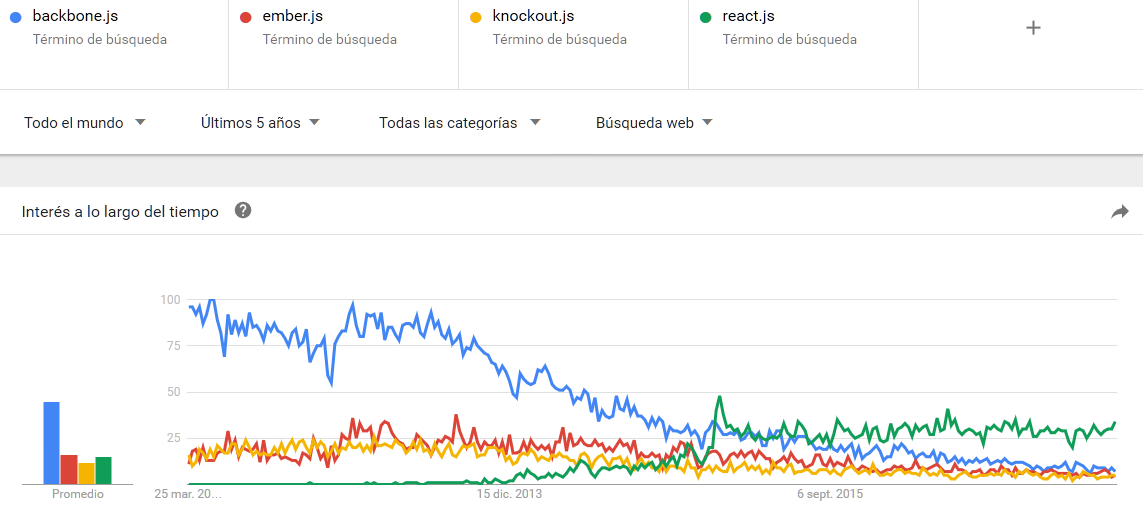
\includegraphics[width=0.8\textwidth]{Figures/ch1/frameworks/graph_frameworks_js_wo_angular}
  \caption{Evolución de las busquedas en Google de los diferentes frameworks.}
\end{figure}

Vemos como hace unos años Backbone.js gozaba de gran popularidad, estando claramente por encima del resto, pero  poco a poco esta popularidad ha ido bajando hasta ponerse al nivel de Knockout.js y EmberJS, los cuales mantienen más o menos el nivel pero también sufren. Por el contrario, React.js, aun siendo el último en llegar, consigue superar a los anteriores. Uno de los motivos de estas variaciones es la evolución que están teniendo las \gls{SPA} y las aplicaciones híbridas. Vemos como Backbone.js y Knockout.js son los que mas han bajado y son a su vez, los menos eficaces para desarrollar páginas complejas.

Si os preguntéis por qué no he añadido Angular al gráfico anterior, debajo de esta línea podéis ver la razón.

\begin{figure}[H]
\centering
  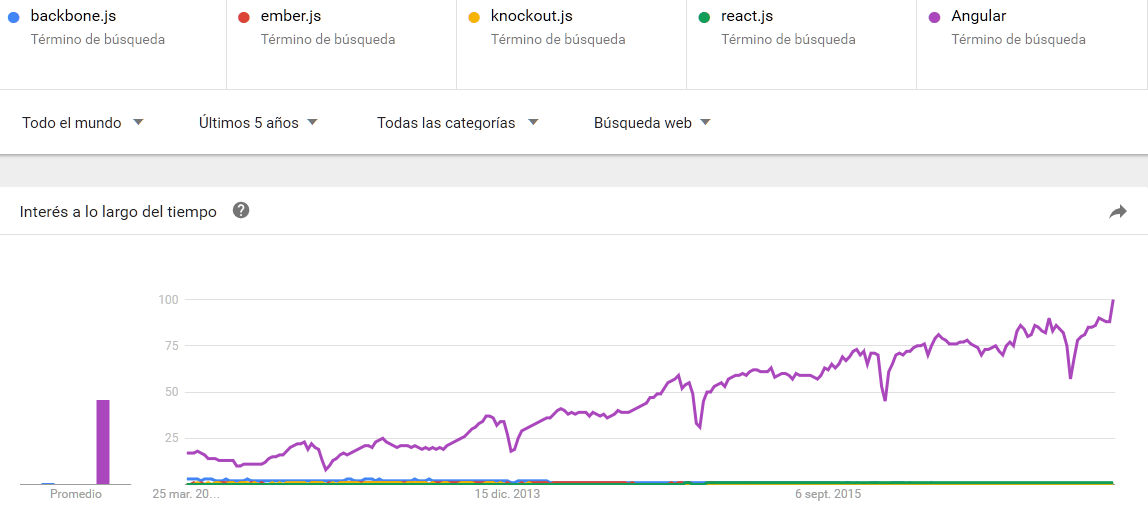
\includegraphics[width=0.8\textwidth]{Figures/ch1/frameworks/graph_frameworks_js_w_angular}
  \caption{La diferencia con Angular es tal, que impide ver correctamente los datos del resto de frameworks.}
\end{figure}

\subsection{Frameworks para aplicaciones híbridas}

\cite{Top10FramHybApp,TopFramHybApp} Junto a la aparición de las aplicaciones híbridos han ido aparecido nuevas necesidades. Como se ha visto en la \nameref{ch:introduction}, el fuerte de estas aplicaciones es la posibilidad de crear una aplicación que funcione en diferentes tipos de dispositivos a partir de un único desarrollo. La variedad de dispositivos, no solo si tenemos en cuenta la plataforma en la que se basa, si no también las características del hardware (en especial el tamaño y la resolución de la pantalla) puede suponer un problema a la hora de realizar el diseño de nuestra aplicación. Por otro lado, este tipo de aplicaciones suelen tener cierta complejidad, ya que suelen estar compuestas por diferentes vistas, utilizan servicios en la nube, necesitan comunicarse con la \gls{API} del dispositivo, \ldots.

Surgieron entonces diferentes frameworks que tratan de dar solución a estos problemas. Algunos de ellos pensados para crear aplicaciones web que se vieran bien en los navegadores móviles, pero que se han usado a la hora de crear aplicaciones híbridas, y otros cuyo único objetivo es servir para el desarrollo de estas últimas. Obviando tanto \emph{Apache Cordova} como \emph{Ionic} ya que hablaremos de ellos más adelante, los más destacables son:

\begin{enumerate}
  \item jQuery Mobile: El abuelo de los framework para dispositivos móviles. Se trata de una versión mínima de jQuery UI y que como no, se apoya sobre jQuery. Se trata de un framework ligero cuyo objetivo principal es funcionar en el mayor número posible de terminales sin importar la plataforma, el tamaño o el navegador usado. Tiene su propio estilo, sin adaptarse al \emph{look and feel} de la plataforma que lo ejecuta, lo que es una limitación importante si queremos decidirnos por él. Aunque no lo incorpora por defecto, es compatible con Apache Cordova.
  \item Appcelerator Titanium: Este framework no sirve para crear aplicaciones híbridas tal como las hemos definido, pero es importante también nombrarlo debido a la popularidad con la que cuenta. A diferencia de \emph{Apache Cordova}, que como veremos más adelante, utiliza un una WebView sobre la cual corre la aplicación web, \emph{Appcelerator} traduce el código JavaScript al código nativo de la plataforma. La interfaz gráfica se crea desde el propio \gls{JS}. Solo se encuentran disponibles las plataformas Android y iOS, que aunque menor, puede ser un inconveniente en según que proyecto. Además, el código a utilizar en Android y en iOS presentan algunas diferencias, lo que nos puede llevar a a tener que mantener dos códigos, aunque con variaciones mínimas entre ellos.
  \item React Native: Este framework esta apoyado por Facebook, quien lo creo y libero hace unos años. React Native no se basa \emph{Apache Cordova} como hace \emph{Ionic}, si no que ejecuta el código \gls{JS} de la aplicación utilizando el motor Javascript de la plataforma (V8 en Android, Javascript Core en iOS) y a medida que se va ejecutando la aplicación, un interprete lee el código \gls{HTML} y crea una vista nativa según este. Esto le proporciona la ventaja de que los elementos que se ven en realidad son nativos, haciendo que se vean mejor que los que generan otros frameworks que se basan en "imitarlos" usando estilos \gls{CSS}.
  \item NativeScript: Similar a React Native en cuanto a funcionamiento, pero permitiendo además el uso de TypeScript y Angualar2 para programar nuestra aplicación y no tener que estar limitados al uso de ReactJS. Un inconveniente que tiene respecto a React Native es la empresa que está detrás. Mientras que ReactJS cuenta con Facebook a sus espaldas, NativeScript está soportado Telerik, que sin querer menospreciarles, no poseen el mismo empuje con el que cuenta el anterior.
  \item Framework 7: Por último nos encontramos con Framework 7, el cual se centra únicamente en iOS y en Android. Permite la creación de aplicaciones híbridas usando PhoneGap, o de WebApps, es decir, aplicaciones que se ejecutan en el navegador, pero manteniendo el aspecto visual de la plataforma donde se ejecuta.
\end{enumerate}

\tipbox{El término \textbf{look and feel} se refiere al aspecto y comportamiento que presenta una interfaz gráfica de cara al usuario. Por lo general, una aplicación o sistema cuentan con una serie de características visuales (paleta de colores, tipo y tamaño de letra, animaciones, iconos, \ldots) que el usuario es capaz de reconocer como propio de esta aplicación o sistema.}

Como en los anteriores frameworks, podemos comprobar la popularidad de los comentados según sus búsquedas en Google.

\begin{figure}[H]
\centering
  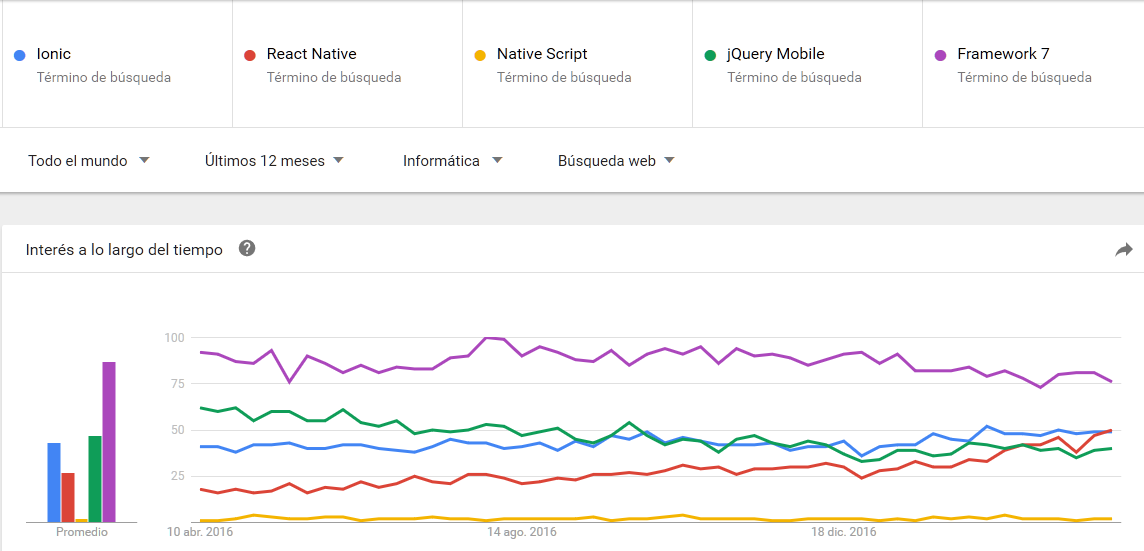
\includegraphics[width=0.8\textwidth]{Figures/ch1/frameworks/graph_frameworks_hyb}
  \caption{Vemos como quitando Framework 7 y NativeScript, el resto de frameworks están a la par.}
\end{figure}

Hay que decir que tanto Framework 7 como jQuery Mobile también son usados para la creación de WebApps y de paginas web con aspecto \emph{responsive}, por lo que cuentan con cierta ventaja a la hora de hablar de popularidad. Si miramos por foros y en diversas comunidades de desarrolladores, parece que las opciones preferidas a la hora de crear aplicaciones híbridas son Ionic y React Native.
